\documentclass{beamer}

\usepackage{amsmath}
\usepackage{textcomp}
\usepackage{listings}
\usepackage{lmodern}
\usepackage{hyperref}
\usepackage[T1]{fontenc}
\usepackage{tikz}
\usepackage{anyfontsize}

\usepackage[disable]{todonotes}

% Required for biblatex, but also adds functionality for quotation
\usepackage{csquotes}

% Jason's bibliography format
% % Credit to Gabriel Devenyi for this bibliography cfg:
% % github.com/gdevenyi/mcmaster.latex
% \usepackage[
%   style=numeric-comp,
%   backend=biber,
%   sorting=none,
%   backref=true,
%   maxnames=99,
%   alldates=iso,
%   seconds=true
% ]{biblatex} % bibliography
% \addbibresource{references.bib}
\usepackage[round]{natbib}
\bibliographystyle{plainnat}
\setcitestyle{yysep={;}}
\defcitealias{ISTQB}{Hamburg and Mogyorodi}
\newcommand{\citetISTQB}{\citetalias{ISTQB} (\citeyear{ISTQB})}
\newcommand{\citepISTQB}{\citepalias[\citeyear{ISTQB}]{ISTQB}}
\newcommand{\citealpISTQB}{\citetalias{ISTQB}, \citeyear{ISTQB}}

% For directory trees
\usepackage{dirtree}

\lstset{
    language=[latex]tex,
    breaklines=true}

\usetheme{Madrid}

\setbeamertemplate{caption}{\centering\insertcaption\par}

% Change block width
\addtobeamertemplate{block begin}{%
    \centering\large%
    \setlength{\textwidth}{0.9\textwidth}
}{}

% From https://tex.stackexchange.com/a/489625/192195
\BeforeBeginEnvironment{block}{\begin{adjustbox}{minipage={\linewidth}, center}}
    \AfterEndEnvironment{block}{\end{adjustbox}}

\usepackage{adjustbox}

\def\checkmark{\tikz\fill[scale=0.4](0,.35) -- (.25,0) -- (1,.7) -- (.25,.15) -- cycle;} 

\newif\ifnotpaper

\def\litStd{If software engineering holds code to high standards of clarity,
    consistency, and robustness, the same should apply to its supporting literature!}

\def\badTaxonomies{Unfortunately, a search for a systematic, rigorous, and
    complete taxonomy for software testing revealed that the existing ones are
    inadequate\todo{ProWritingAid suggests that including ``and incomplete'' is redundant}:
    % and incomplete

    \begin{itemize}
        \item \ifnotpaper\else Tebes et al. \fi\citet{TebesEtAl2020a} focus on
              \emph{parts} of the testing process (e.g., test goal, testable entity),
        \item \ifnotpaper\else Souza et al. \fi\citet{SouzaEtAl2017} prioritize
              organizing testing approaches over defining them, and
        \item \ifnotpaper\else Unterkalmsteiner et al. \fi\citet{UnterkalmsteinerEtAl2014}
              focus on the ``information linkage or transfer'' \citetext{p.~A:6}
              between requirements engineering and software testing.
    \end{itemize}}
\notpapertrue

\title[Testing Terminology]{Putting Software Testing Terminology to the Test}
\subtitle{M.A.Sc. Seminar}
\author[Samuel Crawford]{Samuel Crawford, B.Eng.}

% Committee
% \begin{itemize}
%     \item \emph{Supervisor}: Dr.~Jacques Carette
%     \item \emph{Supervisor}: Dr.~Spencer Smith
%     \item Dr.~Ned Nedialkov
%     \item Dr.~Richard Paige
% \end{itemize}

\institute[McMaster University]{McMaster University\\Department of Computing and Software}
\date{Fall 2024}

\AtBeginSection[]
{
  \begin{frame}
    \frametitle{Table of Contents}
    \tableofcontents[currentsection]
  \end{frame}
}

\begin{document}

% From https://tex.stackexchange.com/a/42826/192195
\NewDocumentCommand{\ShowListingForLineNumber}{s O{1.0} m m}{
    \IfBooleanTF{#1}{\vspace{-#2\baselineskip}}{}
    \lstinputlisting[
        style=MyListStyle,
        linerange={#3-#3},
        firstnumber=#3,
    ]{#4}
}

%%%%%%%%%%%%%%%%%%%%%%%%%%%%%%%%%%%%%%%%%%%%%%%%%%%%%%%%%%%%%%%%%%%%%%%%%%%%%%%
%% TITLE PAGE
%%%%%%%%%%%%%%%%%%%%%%%%%%%%%%%%%%%%%%%%%%%%%%%%%%%%%%%%%%%%%%%%%%%%%%%%%%%%%%%
\frame{\titlepage}

%%%%%%%%%%%%%%%%%%%%%%%%%%%%%%%%%%%%%%%%%%%%%%%%%%%%%%%%%%%%%%%%%%%%%%%%%%%%%%%
%% TABLE OF CONTENTS
%%%%%%%%%%%%%%%%%%%%%%%%%%%%%%%%%%%%%%%%%%%%%%%%%%%%%%%%%%%%%%%%%%%%%%%%%%%%%%%

\begin{frame}
    \frametitle{Table of Contents}
    \tableofcontents
\end{frame}

%%%%%%%%%%%%%%%%%%%%%%%%%%%%%%%%%%%%%%%%%%%%%%%%%%%%%%%%%%%%%%%%%%%%%%%%%%%%%%%
%% INTRODUCTION
%%%%%%%%%%%%%%%%%%%%%%%%%%%%%%%%%%%%%%%%%%%%%%%%%%%%%%%%%%%%%%%%%%%%%%%%%%%%%%%
\section{Introduction}

\subsection{The Need for Standardized Terminology}

\begin{frame}
    \frametitle{The Need for Standardized Terminology}
    \begin{itemize}
        \item Engineering is applied science
        \item Scientific fields use precise terminology
        \item Therefore, the same should be true of software engineering!
        \item <2-> Imagine if other fields used unclear, inconsistent, and
              incorrect terminology:
              \begin{itemize}
                  \item Force
                  \item Isotope
                  \item Phalange
              \end{itemize}
    \end{itemize}
    \begin{block}<3->{}{\litStd{}}
        % \vspace{3mm}
        % \hspace\fill{\small--- Dr.~Jacques Carette}
    \end{block}
\end{frame}

\begin{frame}
    \frametitle{Improved Communication}
    \begin{columns}[T]
        \begin{column}{.5\textwidth}
            \begin{center}
                \huge Interorganizational

                \normalsize Schools, companies, etc.

                \vspace{5mm}

                % Based on code frustratingly generated by ChatGPT
                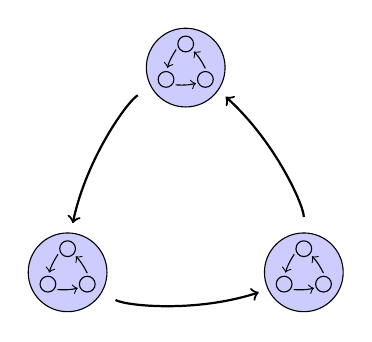
\begin{tikzpicture}

                    % Define coordinates of the triangle's vertices
                    \coordinate (A) at (0, 0);
                    \coordinate (B) at (3, 0);
                    \coordinate (C) at (1.5, 2.6);
                    \coordinate (D) at (1.5, 0.86667);

                    % Draw circles at each vertex without labels
                    \draw[fill=blue!20] (A) circle [radius=0.5];
                    \draw[fill=blue!20] (B) circle [radius=0.5];
                    \draw[fill=blue!20] (C) circle [radius=0.5];

                    % Draw arrows as arcs
                    \draw[->, thick, shorten <= 20pt] (B) arc (0:48:3cm);
                    \draw[->, thick, shorten <= 20pt] (C) arc (120:168:3cm);
                    \draw[->, thick, shorten <= 20pt] (A) arc (240:288:3cm);

                    % Small diagrams inside each circle
                    \only<2->{
                        \foreach \x in {A,B,C} {
                                \begin{scope}[shift={(\x)}, scale=0.2] % Scaling down and shifting to position A
                                    \coordinate (D) at (-1.25, -0.75);
                                    \coordinate (E) at (1.25, -0.75);
                                    \coordinate (F) at (0, 1.5);
                                    \draw[fill=blue!20] (D) circle [radius=0.5];
                                    \draw[fill=blue!20] (E) circle [radius=0.5];
                                    \draw[fill=blue!20] (F) circle [radius=0.5];
                                    \draw[->, shorten <= 4pt] (E) arc (0:45:2.5cm);
                                    \draw[->, shorten <= 4pt] (F) arc (120:165:2.5cm);
                                    \draw[->, shorten <= 4pt] (D) arc (240:285:2.5cm);
                                \end{scope}
                            }
                    }
                \end{tikzpicture}
            \end{center}
        \end{column}
        \begin{column}<2->{.5\textwidth}
            \begin{center}
                \huge Intraorganizational \normalsize
            \end{center}

            \citet[p.~7]{KanerEtAl2011} say ``complete testing'' could require
            the tester to:
            \begin{itemize}
                \item discover ``every bug'',
                \item exhaust the time allocated,
                \item implement every planned test,
                \item \dots{}
            \end{itemize}
        \end{column}
    \end{columns}
\end{frame}

\subsection{The Lack of Standardized Terminology}

\begin{frame}
    \frametitle{The Lack of Standardized Terminology}
    \framesubtitle{``The Problem''}
    \begin{itemize}
        \item \badTaxonomies{}
    \end{itemize}
\end{frame}

\begin{frame}
    \frametitle{Unstandardized Standards}
    \begin{itemize}
        \item The structure of tours is:
              \begin{itemize}
                  \item quite general \citep[p.~34]{IEEE2022}
                  \item<2-> ``organized around a special focus'' \citepISTQB{}
              \end{itemize}
    \end{itemize}
\end{frame}

\begin{frame}
    \frametitle{Unstandardized Standards}
    \begin{itemize}
        \item Load testing is performed with:
              \begin{itemize}
                  \item loads
                        ``between anticipated conditions of low, typical, and
                        peak usage'' \citep[p.~5]{IEEE2022}
                  \item<2-> loads that are as large as possible \citep[p.~86]{Patton2006}
              \end{itemize}
    \end{itemize}
\end{frame}

\begin{frame}
    \frametitle{Unstandardized Standards}
    \begin{itemize}
        \item Alpha testing is performed by:
              \begin{itemize}
                  \item ``users within the organization developing
                        the software'' \citep[p.~17]{IEEE2017}
                  \item<2-> ``a small, selected group of
                        potential users'' \citep[p.~5-8]{SWEBOK2024}
                  \item<3-> ``roles outside the development organization'' conducted
                        ``in the developer's test environment'' \citepISTQB{}
              \end{itemize}
    \end{itemize}

    \begin{block}<4->{}
        {``Okay testing team, we want to conduct alpha testing on our
            product. What's our timeline? Budget? Sample size?''}
        % \vspace{3mm}
        % \hspace\fill{\small--- Dr.~Jacques Carette}
    \end{block}
\end{frame}

%%%%%%%%%%%%%%%%%%%%%%%%%%%%%%%%%%%%%%%%%%%%%%%%%%%%%%%%%%%%%%%%%%%%%%%%%%%%%%%
%% PROJECT
%%%%%%%%%%%%%%%%%%%%%%%%%%%%%%%%%%%%%%%%%%%%%%%%%%%%%%%%%%%%%%%%%%%%%%%%%%%%%%%

\section{Project}
\subsection{Research Questions}

\def\rqa{\begin{alertblock}{Research Question 1}
        \rqatext{}
    \end{alertblock}
}

\def\rqb{\begin{alertblock}{Research Question 2}
        \rqbtext{}
    \end{alertblock}
}

\def\rqc{\begin{alertblock}{Research Question 3}
        \rqctext{}
    \end{alertblock}
}

\begin{frame}{Research Questions}
    \rqa{}\pause
    \rqb{}\pause
    \rqc{}
\end{frame}

%   \begin{figure}
%       %   \vspace{-1mm}
%       \includegraphics[width=.8\textwidth]{assets/stable.png}
%       %   \vspace{-3mm}
%       \caption{Contents of \texttt{stable}}
%       \vspace{-1mm}
%   \end{figure}

%   \lstinputlisting[
%       title=An example log,
%       captionpos=b,
%       language={},
%       basicstyle=\tiny, % TODO: reduce font size?
%       breakatwhitespace=true,
%       showstringspaces=false
%   ]{assets/log.txt}

% \onslide<7-|handout:1>\begin{block}{}
%     {"The information you have should be just as useful for generating
%         tests as it should be for manually running them."}
%     \vspace{3mm}
%     \hspace\fill{\small--- Dr.~Jacques Carette}
% \end{block}


%%%%%%%%%%%%%%%%%%%%%%%%%%%%%%%%%%%%%%%%%%%%%%%%%%%%%%%%%%%%%%%%%%%%%%%%%%%%%%%
%% ACKNOWLEDGEMENTS
%%%%%%%%%%%%%%%%%%%%%%%%%%%%%%%%%%%%%%%%%%%%%%%%%%%%%%%%%%%%%%%%%%%%%%%%%%%%%%%

\begin{frame}
    \frametitle{Acknowledgment}

    \begin{itemize}
        \item Dr.~Smith and Dr.~Carette have been great supervisors in the
              past and have, both then and now, provided me with valuable guidance
              and feedback
              \begin{itemize}
                  \item They have helped me refine the scope of this project
                  \item Dr.~Smith first suggested generating test cases back in 2020!
              \end{itemize}
        \item<2-> The format of this presentation was \emph{heavily} based on
              a previous presentation by Jason Balaci, who also provided a
              great thesis template
        \item<3-> The past and current Drasil team have created a truly amazing
              framework!
    \end{itemize}
\end{frame}

%%%%%%%%%%%%%%%%%%%%%%%%%%%%%%%%%%%%%%%%%%%%%%%%%%%%%%%%%%%%%%%%%%%%%%%%%%%%%%%
%% A FINAL THANK YOU
%%%%%%%%%%%%%%%%%%%%%%%%%%%%%%%%%%%%%%%%%%%%%%%%%%%%%%%%%%%%%%%%%%%%%%%%%%%%%%%

\begin{frame}
    \center
    \huge{Thank you!}\\
    \normalsize{Questions?}
\end{frame}

%%%%%%%%%%%%%%%%%%%%%%%%%%%%%%%%%%%%%%%%%%%%%%%%%%%%%%%%%%%%%%%%%%%%%%%%%%%%%%%
%% REFERENCES
%%%%%%%%%%%%%%%%%%%%%%%%%%%%%%%%%%%%%%%%%%%%%%%%%%%%%%%%%%%%%%%%%%%%%%%%%%%%%%%

% From https://tex.stackexchange.com/a/457255/192195
\setbeamertemplate{page number in head/foot}{}

\begin{frame}[allowframebreaks,noframenumbering]
    \frametitle{References}

    \bibliography{references}
\end{frame}

\end{document}
